\providecommand{\main}{..}
\documentclass[\main/main.tex]{subfiles}
\begin{document}
\subsection{CpGobsExp and CpGperCpG}
The two metric CpGobsExp and CpGperCpG have correlation index 0.9856203442596099.

\begin{figure}
  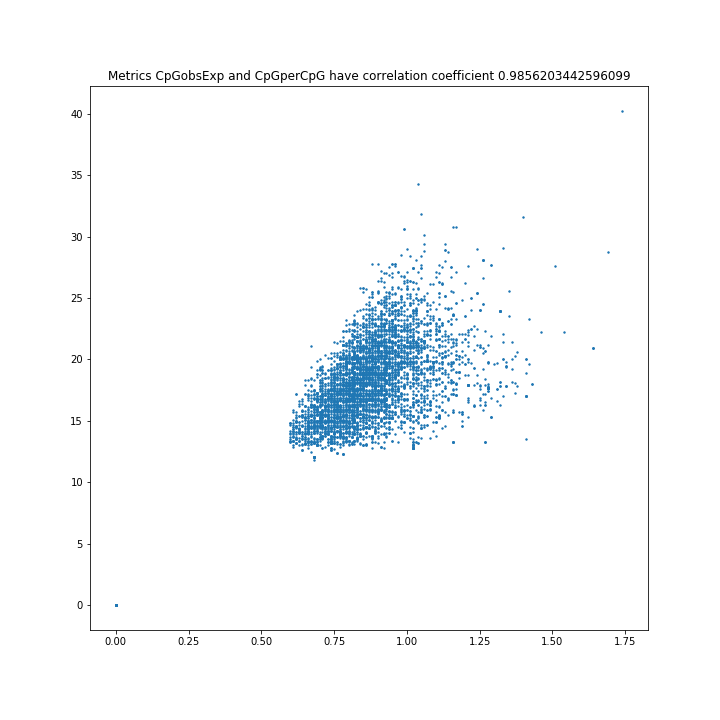
\includegraphics[width=0.5\textwidth]{correlations/CpGobsExp_CpGperCpG}
  \caption{CpGobsExp and CpGperCpG}
\end{figure}

These two metrics have an extremely high correlation, so one of the two will be removed from the dataset, arbitrarily \textbf{CpGobsExp}.

\subsection{CpGobsExp and CpGperGC}
The two metric CpGobsExp and CpGperGC have correlation index 0.9785748818167331.

\begin{figure}
  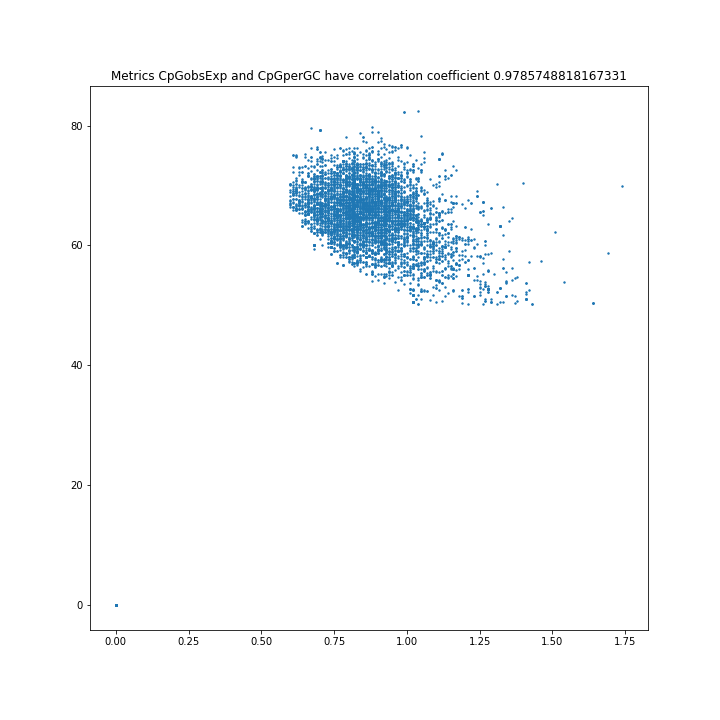
\includegraphics[width=0.5\textwidth]{correlations/CpGobsExp_CpGperGC}
  \caption{CpGobsExp and CpGperGC}
\end{figure}

These two metrics have an extremely high correlation, so one of the two will be removed from the dataset, arbitrarily \textbf{CpGobsExp}.

\subsection{CpGperCpG and CpGperGC}
The two metric CpGperCpG and CpGperGC have correlation index 0.9897887253514923.

\begin{figure}
  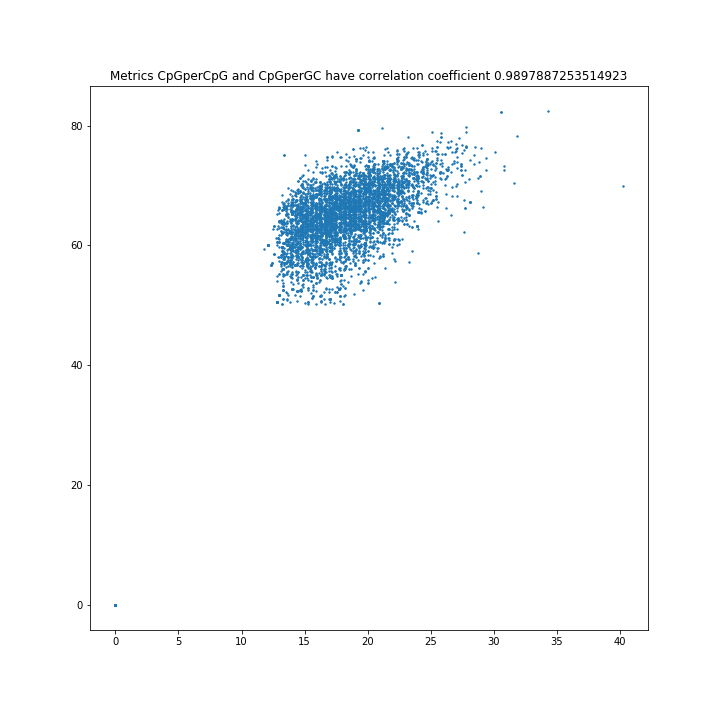
\includegraphics[width=0.5\textwidth]{correlations/CpGperCpG_CpGperGC}
  \caption{CpGperCpG and CpGperGC}
\end{figure}

These two metrics have an extremely high correlation, so one of the two will be removed from the dataset, arbitrarily \textbf{CpGperCpG}.

\subsection{dbVARCount and DGVCount}
The two metric dbVARCount and DGVCount have correlation index 1.0.

\begin{figure}
  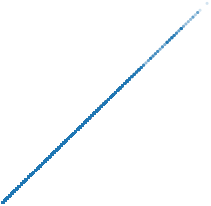
\includegraphics[width=0.5\textwidth]{correlations/dbVARCount_DGVCount}
  \caption{dbVARCount and DGVCount}
\end{figure}

These two metrics have an extremely high correlation, so one of the two will be removed from the dataset, arbitrarily \textbf{dbVARCount}.

\subsection{mamPhyloP46way and verPhyloP46way}
The two metric mamPhyloP46way and verPhyloP46way have correlation index 0.9902257463490804.

\begin{figure}
  
\includegraphics[width=0.5\textwidth]{correlations/mamPhyloP46way_verPhyloP46way}
  \caption{mamPhyloP46way and verPhyloP46way}
\end{figure}

These two metrics have an extremely high correlation, so one of the two will be removed from the dataset, arbitrarily \textbf{mamPhyloP46way}.

\subsection{DnaseClusteredHyp and DnaseClusteredScore}
The two metric DnaseClusteredHyp and DnaseClusteredScore have correlation index 0.7863337778663062.

\begin{figure}
  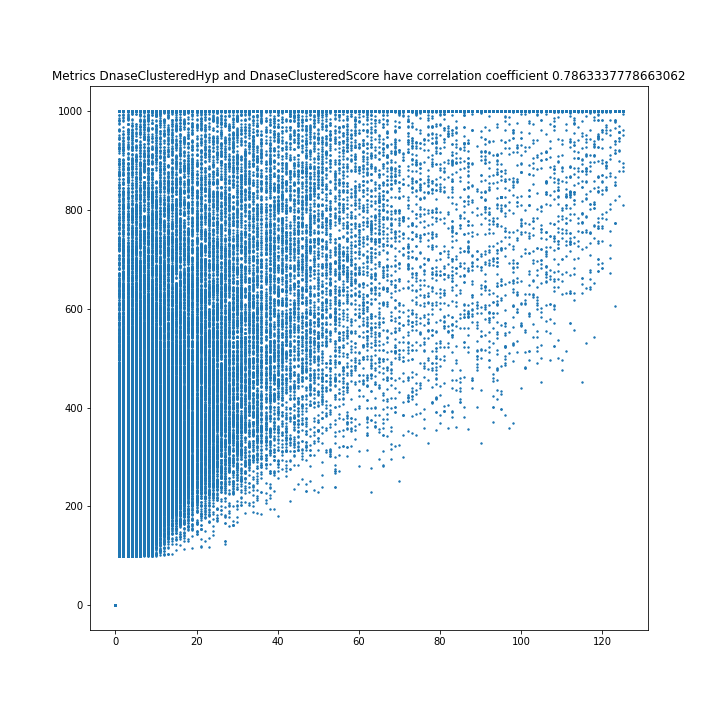
\includegraphics[width=0.5\textwidth]{correlations/DnaseClusteredHyp_DnaseClusteredScore}
  \caption{DnaseClusteredHyp and DnaseClusteredScore}
\end{figure}

The correlation value is high, but not enough to motivate actions such as the removal from the dataset.

\subsection{mamPhastCons46way and verPhastCons46way}
The two metric mamPhastCons46way and verPhastCons46way have correlation index 0.8700263713585867.

\begin{figure}
  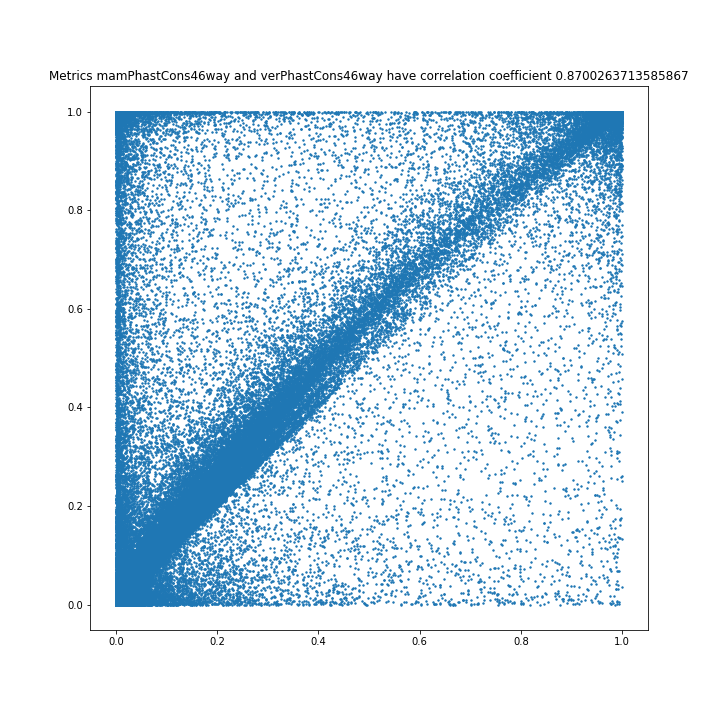
\includegraphics[width=0.5\textwidth]{correlations/mamPhastCons46way_verPhastCons46way}
  \caption{mamPhastCons46way and verPhastCons46way}
\end{figure}

The correlation value is high, but not enough to motivate actions such as the removal from the dataset.

\end{document}